\documentclass{article}

% Language setting
% Replace `english' with e.g. `spanish' to change the document language
\usepackage[T2A]{fontenc}
\usepackage[utf8]{inputenc}

% Set page size and margins
% Replace `letterpaper' with `a4paper' for UK/EU standard size
\usepackage[letterpaper,top=2cm,bottom=2cm,left=3cm,right=3cm,marginparwidth=1.75cm]{geometry}

% Useful packages
\usepackage{amsmath}
\usepackage{graphicx}
\usepackage{float}
\usepackage[colorlinks=true, allcolors=blue]{hyperref}

\title{Лабораторная работа №1}
\author{Выполнили: Цалов В.С. Тахватулин М.В.}

\begin{document}
\maketitle
\begin{center}
      {\fontsize{14}{15}\selectfont
            Преподователь: Оранский С.И.
      }
\end{center}

% \title{Вариант 4}

\section{Задание №1}\label{sec:-no1}


\begin{center}
      \centering
      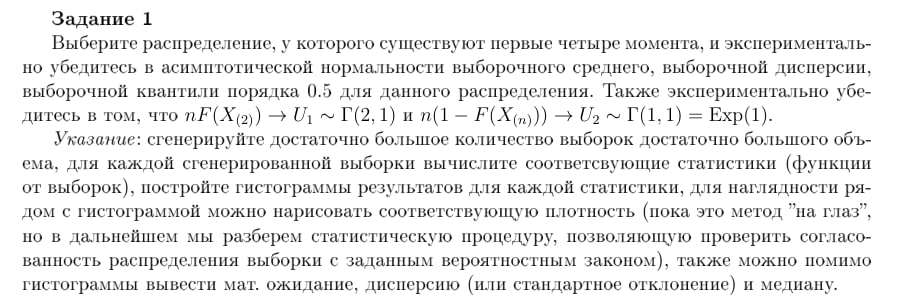
\includegraphics[width=1\linewidth]{1}
\end{center}

\subsection{Выбранное распределение}\label{subsec:-}

В качестве распределения было выбрано распределение хи-квадрат. Со степенью свободы $k = 5$

Гистограмма этого распеределения выглядит примерно так:

\begin{center}
      \centering
      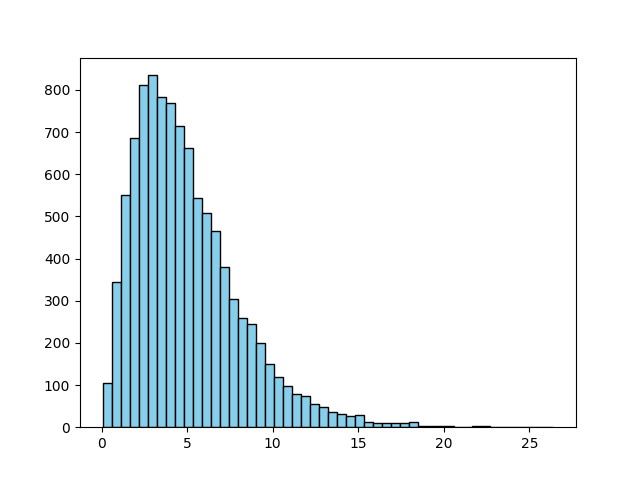
\includegraphics[width=0.5\linewidth]{Python/chi}
\end{center}

\subsection{Первая часть}\label{subsec:-2}
В ходе проведения эксперимента были созданы 1000 выборок по 1000 значений данного распеределения.
В этих выборках были подсчитаны: среднее выборочное значение, выборочная дисперсия и выборочный квантиль порядка 0.5 (медиана выборки)

Гистограммы этих значений
\begin{figure}[H]
      \centering
      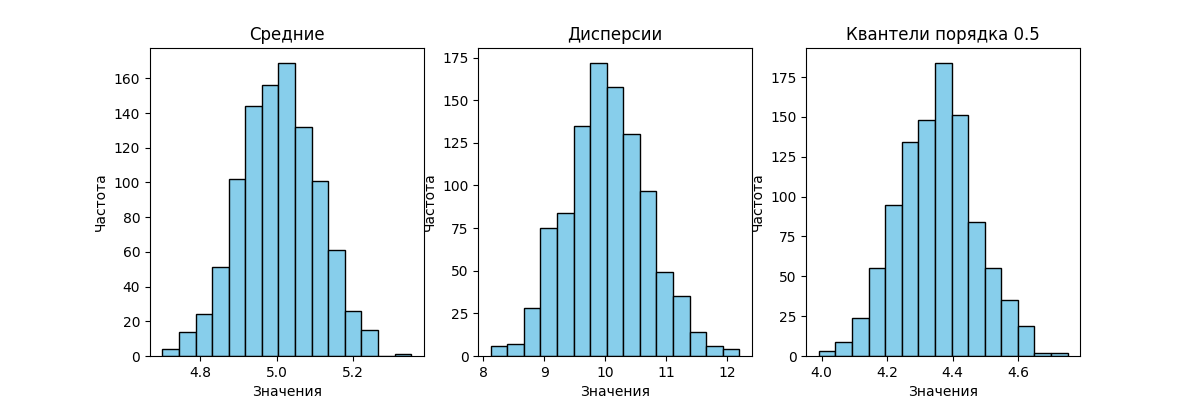
\includegraphics[width=1\linewidth]{Python/first-exp}
      \caption{Гистограммы параметров выборки}\label{fig:figure}
\end{figure}

\subsection{Вывод по первой части}
Изучая полученные графики можно заметить, что они очень похожи на нормальное распределение.

Таким образом можем предположить, что данное задание было направленно на понимание центральной предельной теормы.
Данная теорма заключается в том, что большая выборка независимых величин, подчиняющихся одному и тому же закону распределения, стремится к нормальному.
Что и можно увидеть в этом задании


\subsection{Код}\label{subsec:}
\begin{verbatim}
import numpy as np
import matplotlib.pyplot as plt
#Степень свободы распределения хи квадрат
k = 5

#Массивы значений выборок
E = np.array([])
D = np.array([])
M = np.array([])

#Размеры выборок
counting_samples = 1000
size_sample = 1000

# Получение выборок и их параметров
for i in range(counting_samples):
    if i == 1:
        plt.hist(data, bins=50,  color='skyblue', edgecolor='black')
        plt.xlabel('Значения')
        plt.ylabel('Частота')
        plt.title('Гистограмма выборки по распределению хи-квадрат')
        #plt.savefig('hist-chi-square.png')
        plt.show()
    data = np.random.chisquare(k, size_sample)
    data = np.sort(data)
    # e_loc = sum(data) / 1000
    e_loc = np.mean(data)
    d_loc = np.var(data, ddof=1)
    m_loc = np.median(data)
    M = np.append(M, m_loc)
    D = np.append(D, d_loc)
    E = np.append(E, e_loc)


# Построение графиков
plt.figure(figsize=(12, 4))
plt.subplot(1, 3, 1)
plt.hist(E, bins=15,  color='skyblue', edgecolor='black')
plt.xlabel('Значения')
plt.ylabel('Частота')
plt.title('Средние')
# plt.savefig('hist-mean.png')
plt.show()

plt.subplot(1, 3, 2)
plt.hist(D, bins=15,  color='skyblue', edgecolor='black')
plt.xlabel('Значения')
plt.ylabel('Частота')
plt.title('Дисперсии')
# plt.savefig('hist-disp.png')
plt.show()

plt.subplot(1, 3, 3)
plt.hist(M, bins=15,  color='skyblue', edgecolor='black')
plt.xlabel('Значения')
plt.ylabel('Частота')
plt.title('Квантели порядка 0.5')
# plt.savefig('hist-median.png')
# plt.savefig('first-exp.png')
plt.show()
\end{verbatim}


\subsection{Вторая часть}\label{subsec:---}
Второй эксперимент заключается в том, что нам надо сравнить порядковые статистки с гамма-распределением.

Сортируем каждую выборку для нахождения второй и n-ой порядковой статистики $F(X_{(2)})$ и $F(X_{(n)})$.
Затем находим значения $nF(X_{(2)})$ и $n(1 - F(X_{(n)}))$ и затем заносим их в выборку.
Далее генерируем гамма распределение с параметрами $\Gamma(2, 1)$ и $\Gamma(1, 1)$

В итоге получаем такие графики:

\begin{figure}[H]
      \centering
      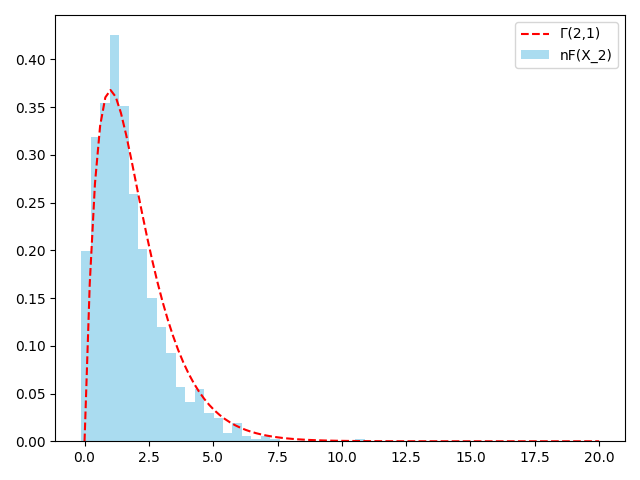
\includegraphics[width=0.5\linewidth]{Python/second-two-one}\label{fig:figure2}
\end{figure}

\begin{figure}[H]
      \centering
      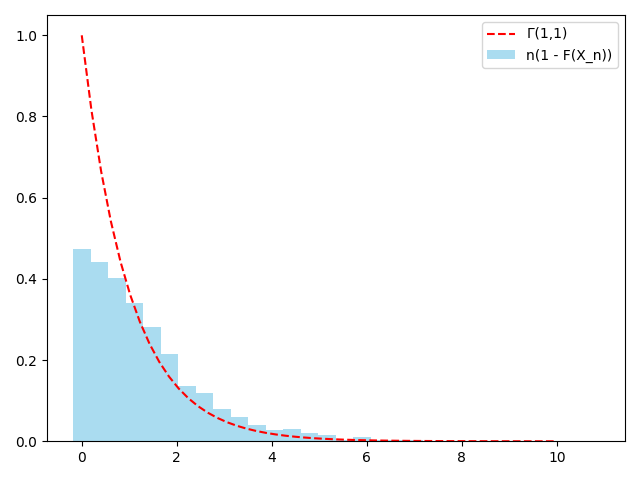
\includegraphics[width=0.5\linewidth]{Python/second-one-one}\label{fig:figure3}
\end{figure}

\subsection{Вывод по второй части}
Изучая полученные графики, можно увидеть, что распределение порядковых статистик подчинено гамма закону распределения.

Таким образом мы проверили теорему о порядковых статистиках,
которая говорит о том, что порядковые статистики имеют гамма распределение.


\subsection{Код второй части}\label{subsec:--}
\begin{verbatim}
import numpy as np
import matplotlib.pyplot as plt
from scipy.stats import gamma, chi

# Параметры гамма распределения
shape = 2
rate = 1

# Нахождение второй порядковой статистики
distrib_func_values = []
values = []
for i in range(1000):
    distribution = chi(4)
    samples = np.sort(distribution.rvs(1000))
    sec_value = samples[1]
    distrib_func_value = (distribution.cdf(sec_value) * 1000)
    values.append(distrib_func_value)
distrib_func_values.append(values)

hist, bins = np.histogram(distrib_func_values, bins=30, density=True)
plt.bar(bins[:-1], hist, width=np.diff(bins), color='skyblue', alpha=0.7, label='nF(X_2)')

# Гамма распределение
x = np.linspace(0, 20, 100)
y = gamma.pdf(x, a=shape, scale=1 / rate)

# Посторение графика
plt.plot(x, y, color='red', linestyle='--', label='Г(2,1)')
plt.legend()
plt.tight_layout()
# plt.savefig('second-two-one.png')
plt.show()



# Нахождение последней порядковой статистики
for i in range(1000):
    distribution = chi(4)
    samples = np.sort(distribution.rvs(1000))
    last_value = samples[-1]
    distrib_func_value = ((1 - distribution.cdf(last_value)) * 1000)
    values.append(distrib_func_value)
distrib_func_values.append(values)

hist, bins = np.histogram(distrib_func_values, bins=30, density=True)
plt.bar(bins[:-1], hist, width=np.diff(bins), color='skyblue', alpha=0.7, label='n(1 - F(X_n))')

# Новые параметры гамма распеределения
shape = 1
rate = 1

# Построение гамма распределения
x = np.linspace(0, 10, 50)
y = gamma.pdf(x, a=shape, scale=1 / rate)

# Построение графика
plt.plot(x, y, color='red', linestyle='--', label='Г(1,1)')
plt.legend()
plt.tight_layout()
plt.savefig('second-one-one.png')
plt.show()
\end{verbatim}

\section{Задание №2. Вариант 4}\label{sec:-no2.--4}

\begin{center}
      \centering
      
\includegraphics[width=1\linewidth]{2}
\end{center}

\subsection{Выполнение}\label{subsec:2}
Из данных надо было найти количество телефонов с различными параметрами.

Итог:
Количество моделей с двумя симкартами: 1019

Количество моделей поддерживающих 3g: 1523

Наибольшее число ядер у процессора: 8

Далeе надо было посчитать параметры выборки телефонов:

Выборочное среднее емкости аккумулятора: 1238.5185

Выборочная дисперсия емкости аккумулятора: 193088.35983766883

Выборочная медиана емкости аккумулятора: 1226.0

Выборочная квантиль порядка 2/5 емкости аккумулятора: 1076.0

Построить графики.
Эмперические функции:
\begin{figure}[H]
      \centering
      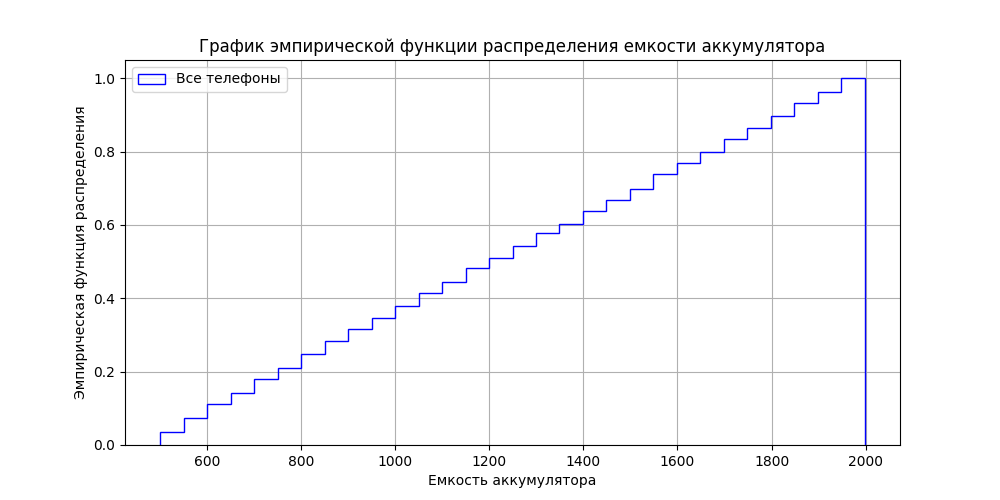
\includegraphics[width=0.5\linewidth]{Python/emper-all-phones}\label{fig:figure4}
\end{figure}

\begin{figure}[H]
      \centering
      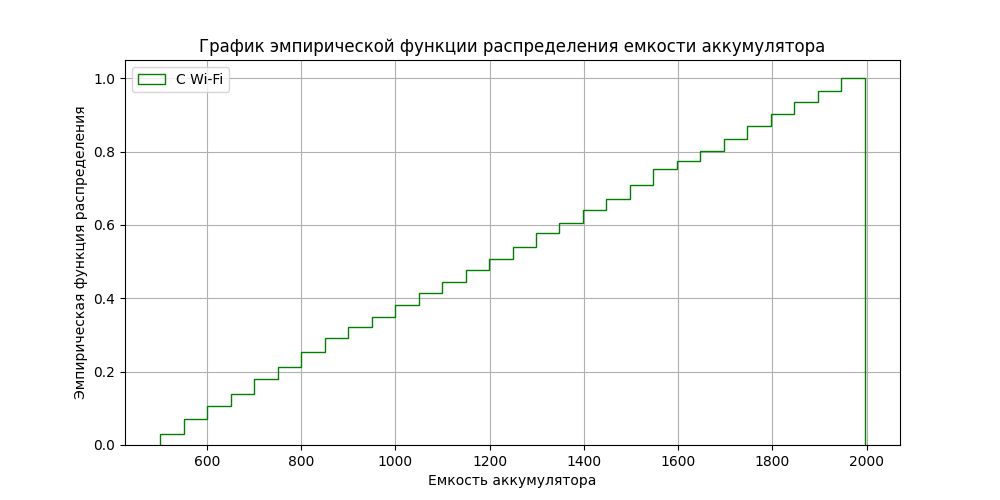
\includegraphics[width=0.5\linewidth]{Python/emper-wi-fi}\label{fig:figure5}
\end{figure}

\begin{figure}[H]
      \centering
      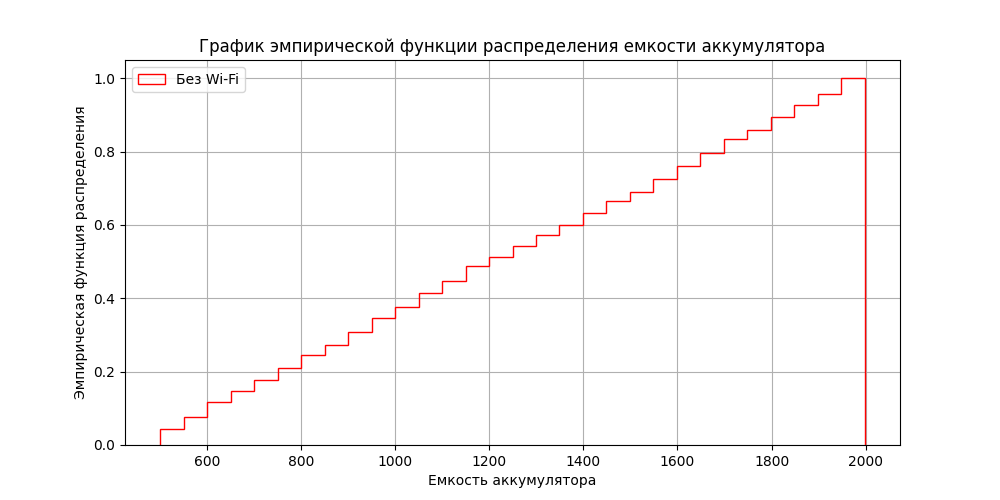
\includegraphics[width=0.5\linewidth]{Python/emper-without-wifi}\label{fig:figure6}
\end{figure}

Гистограммы
\begin{figure}[H]
      \centering
      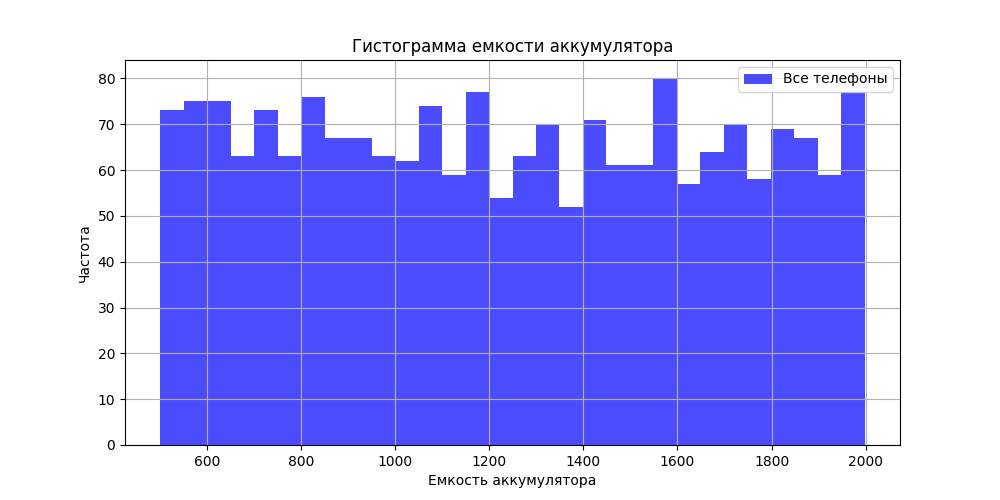
\includegraphics[width=0.5\linewidth]{Python/hist-all-phones}\label{fig:figure7}
\end{figure}

\begin{figure}[H]
      \centering
      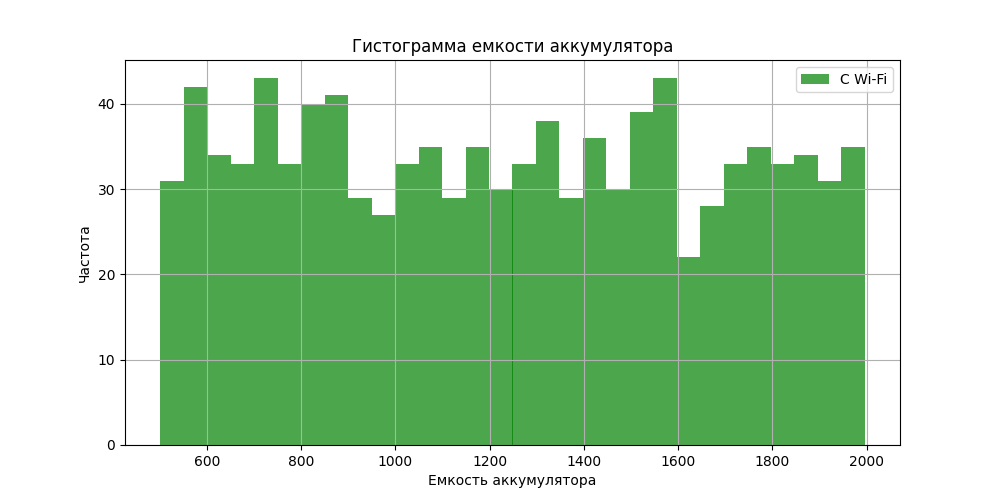
\includegraphics[width=0.5\linewidth]{Python/hist-wi-fi}\label{fig:figure8}
\end{figure}

\begin{figure}[H]
      \centering
      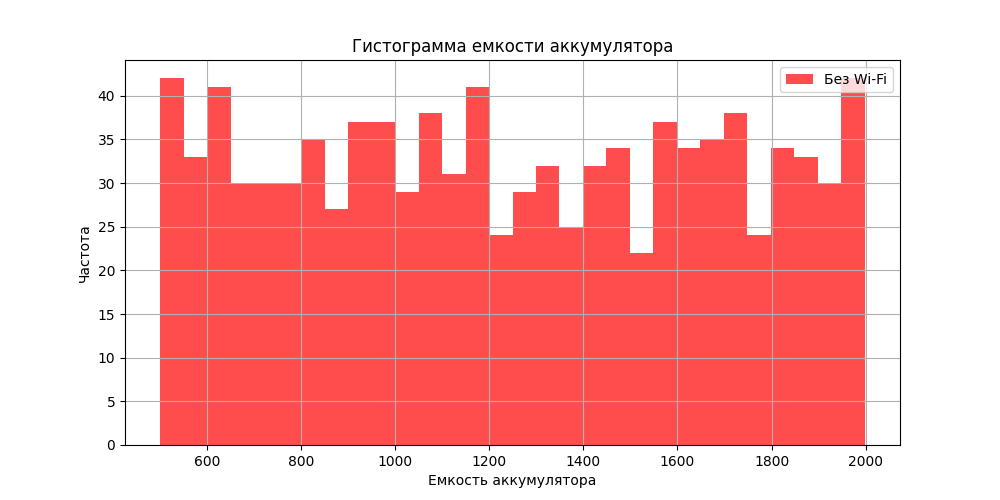
\includegraphics[width=0.5\linewidth]{Python/hist-without-wi-fi}\label{fig:figure9}
\end{figure}

Box-plot:
\begin{figure}[H]
      \centering
      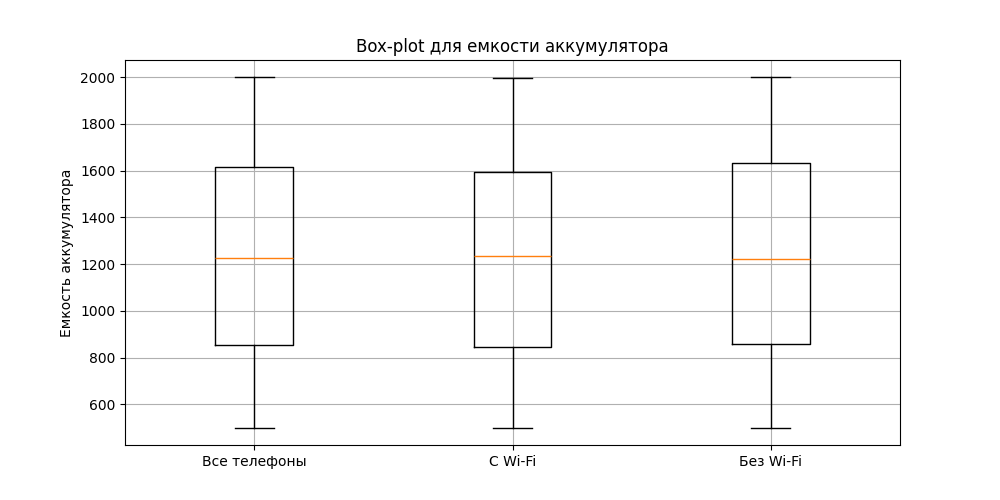
\includegraphics[width=0.5\linewidth]{Python/box-plot}\label{fig:figure10}
\end{figure}

\subsection{Код}\label{subsec:3}
\begin{verbatim}

    import pandas as pd
import matplotlib.pyplot as plt

# Загрузка данных из файла
df = pd.read_csv('mobile_phones.csv', delimiter=",", skiprows=1, names=[
                'battery_power', 'blue', 'clock_speed', 'dual_sim',
                'fc', 'four_g', 'int_memory', 'm_dep', 'mobile_wt', 'n_cores',
                'pc', 'px_height', 'px_width', 'ram', 'sc_h', 'sc_w', 'talk_time',
                'three_g', 'touch_screen', 'wifi', 'price_range'])

print(df[['dual_sim', 'n_cores', 'three_g']])

dual_sim_cnt = sum(df['dual_sim'])
three_g_cnt = sum(df['three_g'] == 1)
max_cores = max(df['n_cores'])

print("Количество моделей с двумя симкартами:", dual_sim_cnt)
print("Количество моделей поддерживающих 3g:", three_g_cnt)
print("Наибольшее число ядер у процессора:", max_cores)

srednee_battery_power = df['battery_power'].mean()
dispersia_battery_power = df['battery_power'].var()
mediana_battery_power = df['battery_power'].median()
kvantil_battery_power = df['battery_power'].quantile(2 / 5)

print("Выборочное среднее емкости аккумулятора:", srednee_battery_power)
print("Выборочная дисперсия емкости аккумулятора:", dispersia_battery_power)
print("Выборочная медиана емкости аккумулятора:", mediana_battery_power)
print("Выборочная квантиль порядка 2/5 емкости аккумулятора:", kvantil_battery_power)


with_wifi = df[df['wifi'] == 1]['battery_power']
without_wifi = df[df['wifi'] == 0]['battery_power']

# empericheskaya func
plt.figure(figsize=(10, 5))
plt.hist(df['battery_power'], bins=30, density=True, cumulative=True,
         histtype='step', label='Все телефоны', color='blue')
plt.xlabel('Емкость аккумулятора')
plt.ylabel('Эмпирическая функция распределения')
plt.title('График эмпирической функции распределения емкости аккумулятора')
plt.legend()
plt.grid(True)
plt.savefig('emper-all-phones.png')
plt.show()

plt.figure(figsize=(10, 5))
plt.hist(with_wifi, bins=30, density=True, cumulative=True,
         histtype='step', label='С Wi-Fi', color='green')
plt.xlabel('Емкость аккумулятора')
plt.ylabel('Эмпирическая функция распределения')
plt.title('График эмпирической функции распределения емкости аккумулятора')
plt.legend()
plt.grid(True)
plt.savefig('emper-wi-fi.png')
plt.show()

plt.figure(figsize=(10, 5))
plt.hist(without_wifi, bins=30, density=True, cumulative=True,
         histtype='step', label='Без Wi-Fi', color='red')
plt.xlabel('Емкость аккумулятора')
plt.ylabel('Эмпирическая функция распределения')
plt.title('График эмпирической функции распределения емкости аккумулятора')
plt.legend()
plt.grid(True)
plt.savefig('emper-without-wifi.png')
plt.show()

# gistogramma
plt.figure(figsize=(10, 5))
plt.hist(df['battery_power'], bins=30, alpha=0.7,
         label='Все телефоны', color='blue')
plt.xlabel('Емкость аккумулятора')
plt.ylabel('Частота')
plt.title('Гистограмма емкости аккумулятора')
plt.legend()
plt.grid(True)
plt.savefig('hist-all-phones.png')
plt.show()

plt.figure(figsize=(10, 5))
plt.hist(with_wifi, bins=30, alpha=0.7,
         label='С Wi-Fi', color='green')
plt.xlabel('Емкость аккумулятора')
plt.ylabel('Частота')
plt.title('Гистограмма емкости аккумулятора')
plt.legend()
plt.grid(True)
plt.savefig('hist-wi-fi.png')
plt.show()

plt.figure(figsize=(10, 5))
plt.hist(without_wifi, bins=30, alpha=0.7,
         label='Без Wi-Fi', color='red')
plt.xlabel('Емкость аккумулятора')
plt.ylabel('Частота')
plt.title('Гистограмма емкости аккумулятора')
plt.legend()
plt.grid(True)
plt.savefig('hist-without-wi-fi.png')
plt.show()

# box plot
plt.figure(figsize=(10, 5))
plt.boxplot([df['battery_power'], with_wifi, without_wifi],
            labels=['Все телефоны', 'С Wi-Fi', 'Без Wi-Fi'])
plt.ylabel('Емкость аккумулятора')
plt.title('Box-plot для емкости аккумулятора')
plt.grid(True)
plt.savefig('box-plot.png')
plt.show()

\end{verbatim}


\end{document}